\chapter{Синтаксис функций}
\label{syntax-in-functions}
\section{Сопоставление с образцом}
\begin{wrapfigure}{r}{0.3\linewidth}
    
\includegraphics[width=1\linewidth]{snail.png}
\end{wrapfigure}
Теперь, когда у нас есть возможность сохранять и компилировать наш код, мы можем начать писать более сложные функции.
Те, что мы написали раньше, были чрезвычайно просты и восторгаться в них было нечем.
Перейдём к более интересным вещам. Первая функция, которую мы напишем, будет выдавать различные приветствия в зависимости от переданного ей пола.
В большинстве языков нужно было бы написать что\--то близкое к этому:
\begin{lstlisting}[style=erlang]
function greet(Gender,Name)
    if Gender == male then
        print("Hello, Mr. %s!", Name)
    else if Gender == female then
        print("Hello, Mrs. %s!", Name)
    else
        print("Hello, %s!", Name)
end
\end{lstlisting}

С использованием сопоставления с образцом, Erlang позволяет избавиться от кучи шаблонного кода.
В Erlang подобная функция будет выглядеть так:
\begin{lstlisting}[style=erlang]
greet(male, Name) ->
    io:format("Hello, Mr. ~s!", [Name]);
greet(female, Name) ->
    io:format("Hello, Mrs. ~s!", [Name]);
greet(_, Name) ->
    io:format("Hello, ~s!", [Name]).
\end{lstlisting}

Признаю, что функция вывода в Erlang выглядит намного уродливее, чем в других языках, но смысл не в этом.
Главное отличие в том, что при использовании сопоставления с образцом, мы убили сразу двух зайцев: определили, какие части функции будут использованы, и связали значения с переменными.
Нам не нужно сначала связывать значения, а потом их сравнивать!
Поэтому вместо:
\begin{lstlisting}[style=erlang]
function(Args)
    if X then
        Expression
    else if Y then
        Expression
    else
        Expression
\end{lstlisting}
Мы напишем:
\begin{lstlisting}[style=erlang]
function(X) ->
    Expression;
function(Y) ->
    Expression;
function(_) ->
    Expression.
\end{lstlisting}

и придём к тем же результатам, используя более декларативный стиль.
Каждое объявление \ops{function} называется \emph{функциональным выражением}.
Функциональные выражения должны разделяться символом точки с запятой (\ops{;}) и вместе они формируют \emph{объявление функции}.
Объявление функции считается одной большой конструкцией, поэтому заключительное функциональное выражение завершается точкой.
Этот способ использования элементов для определения потока задач (workflow), может показаться немного <<странным>>, но вы к нему привыкнете.
Ну или хотя бы надейтесь на то, что это случится, потому что иного пути не существует!\\
\colorbox{lgray}
{
    \begin{minipage}{1\linewidth}
        \textbf{Замечание:} форматирование при помощи \ops{io:format} осуществляется при помощи токенов, которые определяют замены в строке.
        Для обозначения токенов используется символ тильды (\ops{\strut\mytilde}).
        Есть встроенные токены, например\ops{\mytilde n}.
        Этот токен будет преобразован в перевод строки.
        Большинство других токенов обозначают способ форматирования данных.
        Например, вызов функции \ops{io:format(``\mytilde s!\mytilde n'',[``Hello'']).} заключает в себе токен \ops{\mytilde n}, и токен \ops{\mytilde s}, который в качестве аргументов принимает строки и битовые строки.
        После применения форматирования, строка примет вид \ops{``Hello!\\n''}.
        Ещё одним широко используемым токеном является \ops{\mytilde p}.
        Он печатает содержимое переменной Erlang, учитывая форматирование (с добавлением отступов и всего прочего).\\ 
        Мы ознакомимся с подробностями применения функции \ops{io:format} в последующих главах, когда будем углублённо работать с вводом/выводом.
        Но сейчас можете попробовать исполнить следующие вызовы функций: \ops{io:format(''\mytilde s\mytilde n'',[$<<$''Hello''$>>$])}, \ops{io:format''\mytilde p\mytilde n'', [$<<$''Hello''$>>$])}, \ops{io:format(''\mytilde\mytilde\mytilde n'')}, \ops{io:format(''\mytilde f\mytilde n'', [4.0])}, \ops{io:format(''\mytilde 30f\mytilde n'', [4.0])}.
        Это лишь малая часть возможных операций.
        Команды немного похожи на \ops{printf} из другого языка.
        Если не можете дотерпеть до главы, в которой описывается ввод/вывод, то почитайте \href{http://erlang.org/doc/man/io.html\#format-3}{документацию онлайн}.
    \end{minipage}
}

В функциях сопоставление с образцом может принимать ещё более сложные и мощные формы.
Как вы, может быть, помните, несколько глав назад мы применяли сопоставление с образцом, чтобы получать головную и хвостовую части списков.
Давайте попробуем это сделать снова!
Создайте новый модуль и назовите его \ops{functions}.
В нём мы напишем несколько функций, которые позволят нам исследовать пути использования сопоставления с образцом:
\begin{lstlisting}[style=erlang]
-module(functions).
-compile(export_all). %% replace with -export() later, for God's sake!
\end{lstlisting}

Первой нашей функцией станет \ops{head/1}, которая будет вести себя точно так же как \ops{erlang:hd/1}: принимать список в качестве аргумента и возвращать его первый элемент.
Мы будем это делать при помощи оператора cons (\ops{\strut|}):
\begin{lstlisting}[style=erlang]
head([H|_]) -> H.
\end{lstlisting}

Если вы введёте в оболочке \ops{functions:head([1,2,3,4]).} (после того как скомпилируете модуль), то вам будет возвращено значение '1'.
Чтобы получить второй элемент, следовательно, вам нужно создать функцию: 
\begin{lstlisting}[style=erlang]
second([_,X|_]) -> X.
\end{lstlisting}

Список будет разобран Erlang при помощи сопоставления с образцом.
Поробуйте выполнить эту операцию в оболочке!
\begin{lstlisting}[style=erlang]
1> c(functions).
{ok, functions}
2> functions:head([1,2,3,4]).
1
3> functions:second([1,2,3,4]).
2
\end{lstlisting}

Можно повторять этот процесс для списков сколько угодно, но для тысячи значений это было бы непрактично.
Для того чтобы это исправить, мы будем писать рекурсивные функции, которые разберём чуть позже.
А сейчас давайте сосредоточимся на сопоставлении с образцом.
Концепция свободной и связанной переменной, которую мы обсуждали в главе ~\ref{starting-out-for-real}~также справедлива и для функций.
Мы можем сравнивать и выяснять, одинаковы ли два параметра, которые переданы в функцию.
Для этого мы создадим функцию \ops{same/2}, которая принимает два аргумента и сообщает, совпадают ли они друг с другом:
\begin{lstlisting}[style=erlang]
same(X,X) ->
true;
same(_,_) ->
false.
\end{lstlisting}

Вот так всё просто.
Прежде чем объяснять как работают функции, мы ещё раз повторим концепцию связанной и свободной переменной, на всякий случай:
\begin{wrapfigure}{i}{0.7\linewidth}
    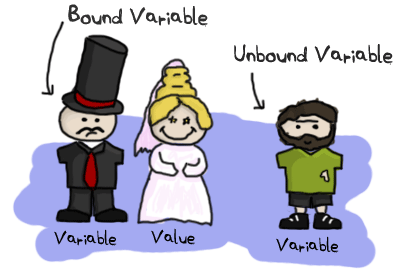
\includegraphics[width=1\linewidth]{un-bound.png}
\end{wrapfigure}
На этой картинке жених опечален, потому что в Erlang переменные никогда не могут менять значение: конец свободе!
А если серьёзно, то свободными называются переменые, у которых ничего нет (как у нашего маленького бомжика справа).
Процесс связывания переменной заключается в простом присоединении значения к свободной переменной.
Если вы захотите присвоить значение связанной переменной, Erlang сгенерирует ошибку.
Но ошибки не будет, если новое значение совпадает со старым.
Представим, что парень слева женится на девушке, у которой есть сестра\--близнец.
Если рядом появится сестра, жених не отличит её от невесты, и никак не отреагирует.
Если же появится посторонняя женщина, жених будет недоволен.
Если вам неясна эта концепция, можете вернуться к разделу о \ref{invariable-variables}~Неизменных переменных.

Вернёмся к нашему коду.
Когда вы вызовете функцию \ops{same(a,a)}, то первая переменная \emph{X} считается свободной и автоматически принимает значение \ops{a}.
Далее Erlang переходит ко второму аргументу, видит что переменная \emph{X} уже связана.
После этого он сравнивает её со значением \ops{a}, которое было передано в качестве второго аргумента, и определяет, совпадают ли они друг с другом.
Операция сопоставления с образцом завершается успешно и функция возвращает \ops{true}.
Если два значения различаются, то сравнение завершится неудачей, и управление перейдёт к второму функциональному выражению, которое не проверяет аргументы (когда выбирать не из чего, нечего перебирать!), а просто возвращает false.
Заметьте, что эта функция может фактически принимать абсолютно любые аргументы! Она работает не только со списками или с одиночными переменными, а с любыми типами данных.
Рассмотрим пример посложнее: функцию, которая печатает дату, но лишь тогда, когда она правильно отформатирована:
\begin{lstlisting}[style=erlang]
valid_time({Date = {Y,M,D}, Time = {H,Min,S}}) ->
    io:format("The Date tuple (~p) says today is: ~p/~p/~p,~n",[Date,Y,M,D]),
    io:format("The time tuple (~p) indicates: ~p:~p:~p.~n", [Time,H,Min,S]);
valid_time(_) ->
    io:format("Stop feeding me wrong data!~n").
\end{lstlisting}

Есть также возможность использовать оператор \ops{\strut=}, который позволяет сопоставлять не только содержимое кортежа (\ops{\{Y,M,D\}}), но и сам кортеж в целом (\emph{Date}).
Функцию можно протестировать следующим образом:
\begin{lstlisting}[style=erlang]
4> c(functions).
{ok, functions}
5> functions:valid_time({{2011,09,06},{09,04,43}}).
The Date tuple ({2011,9,6}) says today is: 2011/9/6,
The time tuple ({9,4,43}) indicates: 9:4:43.
ok
6> functions:valid_time({{2011,09,06},{09,04}}).
Stop feeding me wrong data!
ok
\end{lstlisting}

Правда есть одна проблема!
Эта функция будет принимать в качестве входящих данных что угодно, даже текст или атомы.
Достаточно лишь, чтобы кортежи имели вид \ops{\{\{A,B,C\}, \{D,E,F\}\}}.
Вот мы и пришли к одному из ограничений сопоставления с образцом: с его помощью можно указать либо очень точные значения, например известное число или атом, либо абстрактные значения, такие как голова|хвост списка, кортеж из \emph{N} элементов, или что угодно другое (\ops{\strut\_} и свободные переменные), и т.д.
Чтобы решить эту проблему мы используем охранные выражения, стражи (guards). 
\section{Стража! Стража!}
Стражи \--- это дополнительные выражения, которые можно добавлять в заголовки функций, чтобы сделать сопоставление с образцом более выразительным.
Как уже упоминалось выше, в сопоставлении с образцом есть ограничения, так как с его помощью нельзя сопоставлять, к примеру, диапазон значений, или  определённые типы данных.
Мы не можем выразить концепцию счёта: слишком ли низок этот двенадцатилетний баскетболист, чтобы играть с профессионалами?
Слишком ли велика эта дистанция, чтобы пройти её на руках?
Ты слишком стар, или слишком молод, чтобы водить машину?
На такие вопросы не ответишь, применяя лишь простое сопоставление с образцом.
Конечно, можно представить вопрос про вождение в таком виде:
\begin{lstlisting}[style=erlang]
old_enough(0) -> false;
old_enough(1) -> false;
old_enough(2) -> false;
...
old_enough(14) -> false;
old_enough(15) -> false;
old_enough(_) -> true.
\end{lstlisting}

Но это уж слишком громоздко.
Если хотите, можете так делать, но будьте готовы работать над своим кодом в гордом одиночестве.
Если всё же хотите со временем обзавестись друзьями, создайте новый модуль \ops{guards}, в котором мы реализуем <<правильное>> решение для вопроса о вождении:
\begin{lstlisting}[style=erlang]
old_enough(X) when X >= 16 -> true;
old_enough(_) -> false.
\end{lstlisting}

Вот и всё!
Как видите, такая запись намного короче и понятнее.
Основное правило для охранных выражений: чтобы выражение сработало, оно должно возвращать \ops{true}.
Если страж возвращает \ops{false}, или бросает исключение, то оно не срабатывает.
Предположим, что мы хотим запретить садиться за руль людям старше 104 лет.
Водить можно только в возрасте от 16 до 104 лет. Как же нам выполнить это условие?
Давайте просто добавим второе охранное выражение:
\begin{lstlisting}[style=erlang]
right_age(X) when X >= 16, X =< 104 ->
    true;
right_age(_) ->
    false.
\end{lstlisting}

Запятая (\ops{\strut,}) по выполняемой роли похожа на оператор\ops{andalso}, а точка с запятой (\ops{;}) ведёт себя приблизительно как\ops{orelse} (эти операторы описаны в разделе \ref{boolandcompare}~Булева алгебра и операторы сравнения).
Чтобы всё выражение успешно выполнилось, необходимо чтобы было удовлетворено условие в обоих охранных выражениях.
Также можно поменять условия в функции на противоположные:
\begin{lstlisting}[style=erlang]
wrong_age(X) when X < 16; X > 104 ->
    true;
wrong_age(_) ->
    false.
\end{lstlisting}
\begin{wrapfigure}{l}{0.2\linewidth}
    
\includegraphics[width=1\linewidth]{guard.png}
\end{wrapfigure}

И с этим выражением мы всё равно получим правильные результаты.
Если хотите, можете протестировать (вы всегда должны всё проверять!).
В охранных выражениях точка с запятой (\ops{;}) ведёт себя как оператор\ops{orelse}: если первый страж не исполняется, то исполнение переходит ко второму, потом к следующему, до тех пор пока хотя бы один страж возвратит истину или все стражи возвратят ложь.

Помимо функций сравнения и булевых операторов, можно использовать и другие функции, включая математические операции (\ops{A*B\//C >= 0}) и функции определения типа, такие как \ops{is\_integer/1}, \ops{is\_atom/1}, и т.д. (мы вернёмся к ним в следующей главе).
Одним из недостатков охранных выражений является то, что они не принимают функции определённые пользователем из\--за возможных побочных эффектов.
Erlang не чистый функциональный язык программирования, (коим является, к примеру, \href{http://learnyouahaskell.com}{Haskell}) потому что во многом полагается на побочные эффекты: можно выполнять операции ввода\--вывода, пересылать между акторами сообщения, выбрасывать исключения когда угодно и где угодно.
Не существует простого способа определить, что функция, которая используется в охранном выражении, печатает текст.
А может быть не печатает.
А может быть она перехватывает важные сообщения об ошибках при тестировании в нескольких функциональных выражениях.
Поэтому Erlang просто вам не доверяет (и, скорее всего, правильно делает!)

После всего сказанного, у вас должно было появиться понимание базового синтаксиса охранных выражений, достаточное для того чтобы не теряться при встрече с ними.\\
\colorbox{lgray}
{
    \begin{minipage}{\linewidth}
        \textbf{Замечание:} я сравнивал символы \ops{,} и \ops{;} в охранных выражениях с операторами \ops{andalso} и \ops{orelse}.
        По правде говоря, они не совсем эквивалентны.
        Первые будут захватывать возникающие исключения, а вторые не будут.
        Это означает, что если в первой части охранного выражения \ops{X $>=$ N; N $>=$ 0} будет сгенерирована ошибка, то вторая часть всё же будет исполнена, и выражение может сработать.
        Если ошибка была выброшена в первой части выражения \ops{X $>=$ N orelse N $>=$ 0}, то вторая часть будет пропущена, и всё охранное выражение не сработает.\\ 
        Однако (всегда есть какое\--нибудь <<однако>>) только операторы \ops{andalso} и \ops{orelse} могут помещаться в охранное выражение.
        Это означает, что \ops{(A orelse B) andalso C} это валидное выражение, а \ops{(A; B), C} \--- нет.
        Нужно учитывать их различное назначение и использовать в сочетании друг с другом.
    \end{minipage}
}

\section{Что ещё за <<If>>?!}
\ops{If}\--ы ведут себя подобно охранным выражениям и имеют тот же синтаксис, но используются за пределами заголовка функции.
Они даже называются \emph{Охранными шаблонами}.
\ops{if}\--ы в Erlang отличаются от \ops{if}\--ов в большинстве других языков.
По сравнению с ними, это странные создания, которых принимали бы охотнее, называйся они иначе.
Вступая в страну Erlang, оставьте всё что вы знаете об \ops{if} на пороге.
Займите своё место \--- мы отправляемся в путешествие.

Чтобы понять как похожи выражения \ops{if} на охранные выражения, взгляните на следующие примеры:
\begin{lstlisting}[style=erlang]
-module(what_the_if).
-export([heh_fine/0]).
 
heh_fine() ->
    if 1 =:= 1 ->
        works
    end,
    if 1 =:= 2; 1 =:= 1 ->
        works
    end,
    if 1 =:= 2, 1 =:= 1 ->
        fails
    end.
\end{lstlisting}
Сохраним этот код в файл \ops{what\_the\_if.erl}, и попробуем его исполнить:
\begin{lstlisting}[style=repl]
1> c(what_the_if).
./what_the_if.erl:12: Warning: no clause will ever match
./what_the_if.erl:12: Warning: the guard for this clause evaluates to 'false'
{ok,what_the_if}
2> what_the_if:heh_fine().
** exception error: no true branch found when evaluating an if expression
    in function  what_the_if:heh_fine/0
\end{lstlisting}
Ой!
Компилятор нас предупреждает, что условие if в строке 12 (\ops{1 =:= 2, 1 =:= 1}) никогда не будет использовано, так как его единственное охранное выражение всегда возвращает \ops{false}.
Помните, в Erlang всё должно что\--то возвращать, и \ops{if}\-- выражения не являются исключением из этого правила. 
\begin{figure}[h!]
    \centering
    
\includegraphics[width=0.3\linewidth]{labyrinth.png}
\end{figure}
Таким образом, когда Erlang не может найти случай, в котором страж успешно выполнится, будет сгенерирована ошибка: возвращать в этом случае нечего.
Поэтому мы должны добавить ветвь, которая будет успешно исполняться не смотря ни на что.
В большинстве языков это бы называлось 'else'.
В Erlang мы используем слово 'true' (это объясняет, почему VM сгенерировала сообщение <<no true branch found>>)
\begin{lstlisting}[style=erlang]
oh_god(N) ->
    if N =:= 2 -> might_succeed;
        true -> always_does  %% this is Erlang's if's 'else!'
    end.
\end{lstlisting}

Если мы теперь протестируем эту новую функцию (старая будет продолжать плеваться предупреждениями.
Можно их игнорировать или оставить как напоминание о том, как делать нельзя):
\begin{lstlisting}[style=erlang]
3> c(what_the_if).
./what_the_if.erl:12: Warning: no clause will ever match
./what_the_if.erl:12: Warning: the guard for this clause evaluates to 'false'
{ok,what_the_if}
4> what_the_if:oh_god(2).
might_succeed
5> what_the_if:oh_god(3).
always_does
\end{lstlisting}

Вот ещё одна функция, которая показывает как использовать несколько стражей в \ops{if}\--выражении.
Эта же функция также демонстрирует, что любое выражение должно что\--нибудь возвращать: к переменной \emph{Talk} привязывается результат выражения \ops{if} и затем конкатенируется в строку, которая входит в состав кортежа.
Читая код, легко увидеть как отсутствие ветки \ops{true} могло бы всё испортить, если учитывать, что в Erlang не существует такого понятия как null\--значение (как nil в lisp, NULL в C, None в Python и т.д.):
\begin{lstlisting}[style=erlang]
%% note, this one would be better as a pattern match in function heads!
%% I'm doing it this way for the sake of the example.
help_me(Animal) ->
    Talk = if Animal == cat  -> "meow";
            Animal == beef -> "mooo";
            Animal == dog  -> "bark";
            Animal == tree -> "bark";
            true -> "fgdadfgna"
        end,
    {Animal, "says " ++ Talk ++ "!"}.
\end{lstlisting}
А теперь попробуем исполнить:
\begin{lstlisting}[style=erlang]
6> c(what_the_if).
./what_the_if.erl:12: Warning: no clause will ever match
./what_the_if.erl:12: Warning: the guard for this clause evaluates to 'false'
{ok,what_the_if}
7> what_the_if:help_me(dog).
{dog,"says bark!"}
8> what_the_if:help_me("it hurts!").
{"it hurts!","says fgdadfgna!"}
\end{lstlisting}
Как и множество программистов на Erlang, вы, должно быть, недоумеваете \--- почему 'true' взяло верх над 'else' в качестве атома для управления потоком исполнения?
В конце концов, 'else' более привычен.
Richard O'Keefe дал в почтовой рассылке Erlang следующий ответ на этот вопрос.
Я привожу его здесь без купюр, потому что сам не смог бы сформулировать лучше:\\
\colorbox{lgray}
{
    \begin{minipage}{\linewidth}
    Может быть 'else' и привычнее, но это не означает, что 'else' это хорошо.
    Я понимаю, что при помощи выражения '; true ->' очень легко получить в Erlang 'else', но результаты двух десятков лет наблюдений за психологией программирования показывают, что ни к чему хорошему это не приведёт.
    Я начал заменять:
\end{minipage}
}
\begin{lstlisting}[style=erlang]
if X > Y -> a()
    ; true  -> b()
if X > Y -> a()
    ; X < Y -> b()
    ; true  -> c()
end
\end{lstlisting}
\colorbox{lgray}
{
    \begin{minipage}{\linewidth}
на
    \end{minipage}
}
\begin{lstlisting}[style=erlang]     
if X > Y  -> a()
    ; X =< Y -> b()
end

if X > Y -> a()
    ; X < Y -> b()
    ; X == Y -> C()
end
\end{lstlisting}
\colorbox{lgray}
{
    \begin{minipage}{\linewidth}
это немного раздражает, когда я \textbf{пишу} код, но чрезвычайно помогает, когда я его \textbf{читаю}.
    \end{minipage}
}

Лучше всего <<избегать>> и 'else' и 'true': \ops{if}\--ы обычно легче читать, когда явно покрываются все логические исходы, без использования выражения, которое <<ловит всё подряд>>.

Как упоминалось ранее, в охранных выражениях можно использовать ограниченный набор функций (мы ещё с ними встретимся в \ref{types-or-lack-thereof}~Типы (или их отсутствие).
Настало время явить подлинную мощь условных операторов Erlang.
Я представляю вам выражение \ops{case}!\\
\colorbox{lgray}
{
    \begin{minipage}{\linewidth}
\textbf{Замечание:} весь ужас, отражённый в названиях функций файла \ops{what\_the\_if.erl}, относится к языковой конструкции \ops{if}, если рассматривать её с точки зрения \ops{if} любого другого языка.
В контексте Erlang эта конструкция оказывается абсолютно логичной, просто её имя сбивает с толку.
    \end{minipage}
}
\section{В случае\ldots если}

Если считать, что выражения \ops{if} похожи на стражей, то \ops{case \ldots of} похоже на заголовок функции в целом.
Для каждого аргумента можно применять сложные выражения сопоставления с образцом и, вдобавок, использовать стражи!

Так как вы уже неплохо знакомы с синтаксисом, нам не понадобится много примеров.
На этот раз мы напишем функцию дополнения (append) для множеств (sets) (набор уникальных значений), который мы представим как неупорядоченный список.
В смысле эффективности это, пожалуй, наихудшая возможная реализация наборов, но сейчас мы заботимся не об эффективности, а о синтаксисе:
\begin{lstlisting}[style=erlang]
insert(X,[]) ->
    [X];
insert(X,Set) ->
    case lists:member(X,Set) of
        true  -> Set;
        false -> [X|Set]
    end.
\end{lstlisting}
Если мы передаём в функцию пустое множество (список) и терм \emph{X}, она возвращает нам список, который содержит лишь \emph{X}.
Иначе, функция \ops{lists:member/2} проверяет, не является ли элемент частью списка, и возвращает true, если является и false, если нет.
В случае, когда в нашем множестве уже присутствует элемент \emph{X}, нам не нужно изменять список.
Если элемента в списке нет, то мы добавляем \emph{X} первым элементом списка.

В нашем примере, сопоставление с образцом было очень простым.
Оно может усложняться (можете сравнить ваш код с \href{http://learnyousomeerlang.com/static/erlang/cases.erl}{моим}):
\begin{lstlisting}[style=erlang]
beach(Temperature) ->
    case Temperature of
        {celsius, N} when N >= 20, N =< 45 ->
            'favorable';
        {kelvin, N} when N >= 293, N =< 318 ->
            'scientifically favorable';
        {fahrenheit, N} when N >= 68, N =< 113 ->
            'favorable in the US';
        _ ->
            'avoid beach'
    end.
\end{lstlisting}
Здесь представлен ответ на вопрос <<не сходить ли  на пляж?>> для трёх температурных систем: Цельсия, Кельвина и Фаренгейта.
Сопоставление с образцом комбинируется со стражами и, в конце концов, возвращает ответ, который удовлетворяет всем вариантам использования.
Как было указано ранее,  выражения \ops{case\ldots of} это практически то же самое, что и группа заголовков функций со стражами.
Мы даже могли бы записать наш код в следующем виде:
\begin{lstlisting}[style=erlang]
beachf({celsius, N}) when N >= 20, N =< 45 ->
    'favorable';
...
beachf(_) ->
    'avoid beach'.
\end{lstlisting}

Это вызывает вопрос: когда нужно использовать \ops{if}, а когда \ops{case \ldots of} или функции для записи условных выражений?
\section{Что же использовать?}
\begin{figure}[h!]
    \centering
    
\includegraphics[width=0.3\linewidth]{coppertone.png}
\end{figure}
На вопрос <<Что же использовать?>>, \--- ответить довольно сложно.
Между вызовами функций и конструкцией \ops{case \ldots of} разница очень невелика.
На самом деле на низком уровне они реализованы одинаково, поэтому с точки зрения производительности они ничем не отличаются.
Различия появляются, когда обрабатывается более чем один аргумент: \ops{function(A,B) -> \ldots end.} может использовать стражи, чтобы сопоставлять  с образцом A и B, тогда как case выражение было бы необходимо сформулировать приблизительно следующим образом:
\begin{lstlisting}[style=erlang]
case {A,B} of
    Pattern Guards -> ...
end.
\end{lstlisting}

Такая форма редко встречается и наверняка застанет читателя врасплох.
В похожих ситуациях правильнее было бы использовать вызов функции.
С другой стороны, функция \ops{insert/2}, которую мы записали ранее, определённо выглядит яснее в своём текущем виде, без прямого вызова функции, которая проходит по веткам \ops{true} или \ops{false}.

Следующий вопрос: зачем тогда вообще использовать \ops{if}, если \ops{case} и функции достаточно гибки, чтобы реализовать \ops{if} посредством стражей?
За \ops{if} стоит простая логика: эта конструкция была добавлена в язык, чтобы иметь возможность использовать стражи, не описывая сопоставления с образцом, когда в них нет необходимости.

Конечно же, всё это относится больше к индивидуальным предпочтениям.
Определённого ответа на этот вопрос не существует.
Эта тема до сих пор время от времени обсуждается сообществом Erlang.
Если ваш код прост для понимания, никто вас бить не будет, какой бы путь вы не избрали.
Как однажды сказал Ward Cunningham: <<Код можно считать ясным, когда вы смотрите на подпрограмму, и она выглядит приблизительно так, как вы и ожидали.>>
